\documentclass[11pt,a4paper]{article}

\usepackage[utf8]{inputenc}
\usepackage[T1]{fontenc}
\usepackage{amsmath,amssymb,amsfonts,amsthm}
\usepackage{graphicx}
\usepackage{hyperref}
\usepackage{cite}
\usepackage{geometry}
\usepackage{booktabs}
\usepackage{microtype}
\usepackage{bm}

\geometry{margin=1in}

\hypersetup{
    colorlinks=true,
    linkcolor=blue,
    citecolor=red,
    urlcolor=cyan,
    pdftitle={Real-Time Tokamak Plasma Equilibrium Reconstruction and Disruption Mitigation via Moment-Space Dimension Reduction},
    pdfauthor={Hyo Eun Ahn}
}

\newtheorem{theorem}{Theorem}
\newtheorem{lemma}[theorem]{Lemma}
\newtheorem{corollary}[theorem]{Corollary}

\title{\textbf{Real-Time Tokamak Plasma Equilibrium Reconstruction and Disruption Mitigation via Moment-Space Dimension Reduction}}

\author{Hyo Eun Ahn\thanks{Email: \texttt{hyo.eun.ahn@proton.me}}}

\date{\today}

\begin{document}

\maketitle

\begin{abstract}
We present a closed-form moment-space framework for reduced-order tokamak plasma equilibrium reconstruction and an offline feasibility study of boundary stabilization. A three-dimensional fourth-order monomial expansion represents the discretized plasma current distribution using 35 spatial moments. A normalized positive reference prior provides a unique affine reconstruction satisfying the prescribed moment constraints when the moment matrix has full row rank. By combining this reconstruction with a precomputed Green-kernel interaction matrix and a fixed-prior weighted polynomial projection, the spatial mesh dimension is eliminated from online evaluation, yielding a $35 \times 35$ affine operator for approximate magnetic-flux coefficients. The formulation establishes exact algebraic moment consistency within the specified discrete model and distinguishes this property from the physical accuracy of the underlying kernel approximation. An illustrative six-state linear feedback model is examined using a quadratic Lyapunov certificate and a bounded-disturbance invariant-set formulation. Reference numerical benchmarks demonstrate microsecond-scale execution of the reduced-order computational kernels, without establishing end-to-end diagnostic, actuator, or facility-level latency. The results provide a mathematical and computational basis for investigating fast equilibrium estimation and boundary-control feasibility. Validation with device-specific magnetic geometry, calibrated coil dynamics, and experimental discharge data remains future work.
\end{abstract}

\noindent\textbf{Keywords:} Tokamak Equilibrium, Disruption Mitigation, Moment Approach, Dimension Reduction, MHD Stability, Real-time Feedback Control.

---

\section{Introduction}
Magnetic confinement fusion in tokamak devices relies on the precise, continuous confinement of high-temperature hydrogen isotope plasmas by magnetic fields generated by external superconducting coils and internally driven toroidal plasma currents~\cite{wesson2011tokamaks}. A paramount operational challenge confronting contemporary tokamaks such as KSTAR~\cite{kstar2020} and the international thermonuclear experimental reactor (ITER)~\cite{iter2019} is the phenomenon of major disruptions. Disruptions are abrupt, catastrophic terminations of plasma confinement caused by macroscopic magnetohydrodynamic (MHD) instabilities, including vertical displacement events (VDEs), resistive wall modes (RWMs), and neoclassical tearing modes (NTMs)~\cite{hender2007disruptions}. During a disruption, the thermal energy ($\sim 100\,\mathrm{MJ}$ in ITER) and magnetic energy are dumped onto plasma-facing components within 1 to 10 milliseconds, inducing severe thermal ablation and tremendous electromagnetic forces capable of causing structural damage.

Preventing disruptions necessitates real-time active magnetic feedback control operating on sub-millisecond timescales ($\le 1\,\mathrm{ms}$). In standard tokamak control systems (TCS), external magnetic diagnostics---such as flux loops, Rogowski coils, and saddle coils---measure external magnetic signals. The internal plasma state, including the boundary flux contour $\psi_b$, elongation $\kappa$, triangularity $\delta$, and current density profile $J_\phi(R,Z)$, is reconstructed by solving the non-linear Grad-Shafranov equation:
\begin{equation}
    \Delta^* \psi = R \frac{\partial}{\partial R}\left( \frac{1}{R}\frac{\partial \psi}{\partial R} \right) + \frac{\partial^2 \psi}{\partial Z^2} = -\mu_0 R J_\phi(R, \psi) = -\mu_0 R^2 p'(\psi) - \mu_0^2 F(\psi)F'(\psi),
    \label{eq:grad_shafranov}
\end{equation}
where $p(\psi)$ is the plasma pressure, and $F(\psi) = R B_\phi$ is the poloidal current function.

Codes such as EFIT~\cite{lao1985reconstruction} and rtEFIT perform iterative non-linear least-squares minimization over discretized grids ($N \ge 10^3 - 10^4$). Although accelerated variants have been developed, iterative non-linear solvers remain computationally hazardous during rapid transients; when an instability initiates, non-linear convergence can stall, leading to missed control cycles and disruption. On the other hand, ab-initio kinetic tracking (Particle-in-Cell, PIC) tracks millions of individual charged particle trajectories ($\sim O(N^2)$ interactions), requiring supercomputing clusters that are fundamentally incompatible with embedded real-time feedback loops~\cite{birdsall2018plasma}.

In this paper, we extend the foundational moment theory originally conceived in 1994 by the author for space-charge models in particle accelerators~\cite{ahn1994preliminary} to the problem of real-time tokamak equilibrium reconstruction and stabilization. The central philosophy is that macroscopic MHD stability and equilibrium boundary positions depend solely on a finite set of low-order spatial and current moments rather than the infinite microscopic degrees of freedom of individual particles. 

We prove that by introducing a normalized, strictly positive prior distribution vector $\bm{\mu} \in \mathbb{R}^N$ satisfying $\sum_{i=1}^N \mu_i = 1$, the continuous toroidal current distribution in an underdetermined mesh space can be rigorously inverted into an $M$-dimensional monomial moment space ($M=35$ for 4th-order expansions). Crucially, the large dimension $N$ entirely collapses from the runtime execution, leaving a precomputed $M \times M$ matrix multiplication that evaluates in less than $10\,\mu\mathrm{s}$. Furthermore, we examine a Lyapunov-certified LMI stability formulation within an illustrative 6-state linear moment subspace, providing a bounded-disturbance invariant-set certificate within the idealized linear model.

---

\section{Moment-Space Formulation of Tokamak Current Density}

\subsection{Underdetermined Current Reconstruction on Mesh Points}
Consider the poloidal cross-section of a tokamak vessel discretized into $N$ grid points $\bm{r}_i = (R_i, Z_i, \phi_i)$ ($i = 1, \dots, N$). Let $a_i$ represent the effective toroidal current element at mesh point $\bm{r}_i$, and let $\bm{a} = [a_1, a_2, \dots, a_N]^T \in \mathbb{R}^N$. 

The macroscopic state of the plasma is captured by $M$ spatial moments defined over the cross-section:
\begin{equation}
    s_k = \sum_{i=1}^N \Omega_{ki} a_i, \quad k = 1, \dots, M,
    \label{eq:moment_def}
\end{equation}
where $\bm{\Omega} \in \mathbb{R}^{M \times N}$ is the monomial evaluation matrix whose elements are given by $\Omega_{ki} = m_k(\bm{r}_i)$. For a complete expansion up to fourth order in spatial coordinates $(x,y,z)$, there are $M = 35$ distinct monomials:
\begin{equation}
    \bm{m}(\bm{r}) = \left[ 1, x, y, z, x^2, xy, xz, y^2, yz, z^2, x^3, \dots, z^4 \right]^T.
\end{equation}
Because the number of grid points $N \sim 10^3 - 10^5$ far exceeds the number of tracked moments $M = 35$, Eq.~\eqref{eq:moment_def} represents an extremely underdetermined linear system $\bm{s} = \bm{\Omega} \bm{a}$. 

To invert this system and reconstruct a prior-centered moment-consistent current distribution $\bm{a}$ from the moment vector $\bm{s}$, we formulate a constrained quadratic optimization problem. Following the variational approach established by the author in 1994~\cite{ahn1994preliminary}, we minimize the objective functional:
\begin{equation}
    J(\bm{a}) = \frac{1}{2} \sum_{i=1}^N (a_i - \mu_i)^2 + \bm{\lambda}^T (\bm{s} - \bm{\Omega}\bm{a}),
    \label{eq:lagrange_obj}
\end{equation}
where $\bm{\lambda} \in \mathbb{R}^M$ is a vector of Lagrange multipliers, and $\bm{\mu} = [\mu_1, \dots, \mu_N]^T$ is a fixed reference prior distribution. 

\subsection{Elimination of Unphysical Inversion via Normalized Prior}
A pervasive failure mode in standard minimum-norm pseudoinverse reconstructions ($\bm{\mu} = \bm{0}$) is the occurrence of unphysical negative current density values ($a_i < 0$) in the peripheral regions of the plasma boundary, which violates the physical requirement of forward toroidal current drive ($J_\phi \ge 0$).

\begin{theorem}[Closed-Form Charge-Current Distribution]
Let the reference prior vector $\bm{\mu}$ satisfy the normalization condition:
\begin{equation}
    \sum_{i=1}^N \mu_i = 1, \quad \mu_i > 0 \quad \forall i.
    \label{eq:mu_normalization}
\end{equation}
Then, the unique stationary point of the Lagrangian functional~\eqref{eq:lagrange_obj} is given explicitly by:
\begin{equation}
    \bm{a} = \bm{\mu} + \bm{\Lambda} (\bm{s} - \bm{\Omega} \bm{\mu}),
    \label{eq:a_solution}
\end{equation}
where the transformation matrix $\bm{\Lambda} \in \mathbb{R}^{N \times M}$ is defined as:
\begin{equation}
    \bm{\Lambda} = \bm{\Omega}^T (\bm{\Omega} \bm{\Omega}^T)^{-1}.
    \label{eq:lambda_def}
\end{equation}
\end{theorem}

\begin{proof}
Differentiating Eq.~\eqref{eq:lagrange_obj} with respect to $a_i$ and setting the derivative to zero yields:
\begin{equation}
    \frac{\partial J}{\partial a_i} = (a_i - \mu_i) - \sum_{k=1}^M \lambda_k \Omega_{ki} = 0 \implies \bm{a} = \bm{\mu} + \bm{\Omega}^T \bm{\lambda}.
\end{equation}
Multiplying by $\bm{\Omega}$ from the left and enforcing the exact moment constraint $\bm{\Omega}\bm{a} = \bm{s}$:
\begin{equation}
    \bm{\Omega}\bm{a} = \bm{\Omega}\bm{\mu} + (\bm{\Omega}\bm{\Omega}^T)\bm{\lambda} = \bm{s} \implies \bm{\lambda} = (\bm{\Omega}\bm{\Omega}^T)^{-1} (\bm{s} - \bm{\Omega}\bm{\mu}).
\end{equation}
Substituting $\bm{\lambda}$ back into the expression for $\bm{a}$ yields Eq.~\eqref{eq:a_solution}. Under condition~\eqref{eq:mu_normalization}, the baseline zeroth-order state is guaranteed positive everywhere, and the second term acts strictly as a smooth perturbational correction driven by higher-order spatial moments.
\end{proof}

---

\section{Analytical Green's Function Collapse: The Fall-Out of $N$}

\subsection{Polynomial Approximation of the Magnetic Flux Potential}
Having reconstructed the discrete current distribution $\bm{a}$, the exact poloidal magnetic flux function $\psi_{\mathrm{exact}}(\bm{r})$ at any arbitrary field point $\bm{r} = (R,Z)$ is given by the superposition of poloidal Green's functions $G(\bm{r}, \bm{r}_i)$:
\begin{equation}
    \psi_{\mathrm{exact}}(\bm{r}) = \sum_{i=1}^N a_i G(\bm{r}, \bm{r}_i), \quad G(\bm{r}, \bm{r}_i) = \frac{\mu_0}{\pi k} \sqrt{R R_i} \left[ \left(1 - \frac{k^2}{2}\right) K(k) - E(k) \right],
    \label{eq:green_flux}
\end{equation}
where $k^2 = \frac{4 R R_i}{(R + R_i)^2 + (Z - Z_i)^2}$, and $K(k)$, $E(k)$ are complete elliptic integrals of the first and second kind.

In the real-time control system, evaluating Eq.~\eqref{eq:green_flux} over $N$ points is prohibitively slow. We approximate $\psi_{\mathrm{exact}}(\bm{r})$ by a polynomial expansion over the $M$ monomials:
\begin{equation}
    \psi_{\mathrm{approx}}(\bm{r}) = \sum_{j=1}^M v_j m_j(\bm{r}) = \bm{m}^T(\bm{r}) \bm{v},
    \label{eq:psi_approx}
\end{equation}
where $\bm{v} = [v_1, \dots, v_M]^T \in \mathbb{R}^M$ is the coefficient vector to be determined.

To eliminate the mesh dimension $N$ from online computation, we adopt the fixed reference prior $\bm{\mu}$ as the polynomial fitting weight and formulate:
\begin{equation}
    \mathcal{E}_\mu(\bm{v}) = \sum_{i=1}^N \mu_i \left[ \psi_{\mathrm{exact}}(\bm{r}_i) - \psi_{\mathrm{approx}}(\bm{r}_i) \right]^2.
    \label{eq:weighted_lsq_mu}
\end{equation}

\begin{theorem}[Fixed-Prior Dimension Collapse Theorem (The Fall-out of $N$)]
The polynomial coefficient vector $\bm{v}$ minimizing $\mathcal{E}_\mu(\bm{v})$ satisfies:
\begin{equation}
    \bm{v} = \bm{\Lambda}^{\prime T} \bm{D} \bm{\Lambda} \bm{s} + \bm{\Lambda}^{\prime T} \bm{D} \bm{c},
    \label{eq:magic_matrix}
\end{equation}
where $\bm{D} \in \mathbb{R}^{N \times N}$ is the precomputed Green kernel matrix with $D_{ij} = G(\bm{r}_i, \bm{r}_j)$ ($D_{ii} = 0$), $\bm{c} = [\bm{I} - \bm{\Lambda}\bm{\Omega}]\bm{\mu}$, and:
\begin{equation}
    \bm{\Lambda}^{\prime} \equiv \bm{\Lambda}^{\prime}\big|_{\bm{a}=\bm{\mu}} = \bigl\{\bm{\Omega}\bm{\mu}\bigr\}^T \Bigl[ \bm{\Omega} \bigl\{\bm{\Omega}\bm{\mu}\bigr\}^T \Bigr]^{-1}, \quad \{\bm{\Omega}\bm{\mu}\}_{kj} = \Omega_{kj} \mu_j.
    \label{eq:lambda_prime}
\end{equation}
Crucially, the high dimension $N$ is completely eliminated offline, reducing online calculation to an $M \times M$ matrix multiplication.
\end{theorem}

\noindent\textit{Remark (Fixed-Prior Linearization and Surrogate Kernel).}
In the precomputed online operator, $\bm{\Lambda}^{\prime}$ is evaluated at the reference prior $\bm{a} = \bm{\mu}$, yielding a fixed operator $\mathcal{M} = \bm{\Lambda}^{\prime T} \bm{D} \bm{\Lambda}|_{\bm{a}=\bm{\mu}}$ that is an algebraically exact dimension reduction within the fixed-prior linearization. The separate $\bm{a}$-weighted Exact Moment Conservation property (Theorem~3) holds independently for the actual current distribution $\bm{a}$ and does not enter the runtime flux reconstruction path. The numerical benchmarks in Section~5 employ a regularized $1/r$ surrogate interaction kernel to demonstrate the dimensional collapse mechanism; device-specific complete elliptic-integral Green's functions are a direct substitution for machine-specific implementation.

\begin{proof}
Differentiating Eq.~\eqref{eq:weighted_lsq_mu} with respect to $v_k$ ($k=1,\dots,M$):
\begin{equation}
    \frac{\partial \mathcal{E}_\mu}{\partial v_k} = -2 \sum_{i=1}^N \mu_i \left[ \psi_{\mathrm{exact}}(\bm{r}_i) - \sum_{l=1}^M v_l m_l(\bm{r}_i) \right] m_k(\bm{r}_i) = 0.
\end{equation}
In matrix notation, noting that $m_k(\bm{r}_i) = \Omega_{ki}$ and defining the element-wise scaled matrix $\{\bm{\Omega}\bm{\mu}\}_{ki} = \Omega_{ki} \mu_i$:
\begin{equation}
    \{\bm{\Omega}\bm{\mu}\} \bm{\Omega}^T \bm{v} = \{\bm{\Omega}\bm{\mu}\} \bm{\psi}_{\mathrm{exact}}.
    \label{eq:normal}
\end{equation}
Inverting the $M \times M$ matrix on the left-hand side yields:
\begin{equation}
    \bm{v} = \left[ \{\bm{\Omega}\bm{\mu}\} \bm{\Omega}^T \right]^{-1} \{\bm{\Omega}\bm{\mu}\} \bm{\psi}_{\mathrm{exact}} \equiv \bm{\Lambda}^{\prime T} \bm{\psi}_{\mathrm{exact}}.
\end{equation}
Substituting $\bm{\psi}_{\mathrm{exact}} = \bm{D} \bm{a}$ and the expression for current distribution $\bm{a} = \bm{\Lambda}\bm{s} + \bm{c}$ directly yields Eq.~\eqref{eq:magic_matrix}.
\end{proof}

\begin{theorem}[Exact Moment Conservation]
Under the current-weighted least-squares projection with weights $a_i$, the spatial moments of the approximated flux potential exactly equal the moments of the exact flux potential:
\begin{equation}
    \langle m_k \psi_{\mathrm{approx}} \rangle_{\bm{a}} = \langle m_k \psi_{\mathrm{exact}} \rangle_{\bm{a}}, \quad \forall k = 1, \dots, M,
    \label{eq:moment_conservation}
\end{equation}
where the weighted inner product is defined as $\langle f \rangle_{\bm{a}} = \sum_{i=1}^N a_i f(\bm{r}_i)$.
\end{theorem}

\begin{proof}
Expanding the left-hand side of Eq.~\eqref{eq:moment_conservation}:
\begin{equation}
    \langle m_k \psi_{\mathrm{approx}} \rangle_{\bm{a}} = \sum_{i=1}^N a_i m_k(\bm{r}_i) \sum_{l=1}^M v_l m_l(\bm{r}_i) = \left[ \{\bm{\Omega}\bm{a}\} \bm{\Omega}^T \bm{v} \right]_k.
\end{equation}
The $\bm{a}$-weighted optimality condition gives the normal equation $\{\bm{\Omega}\bm{a}\}\bm{\Omega}^T\bm{v} = \{\bm{\Omega}\bm{a}\}\bm{\psi}_{\mathrm{exact}}$. Hence the bracket above identically equals $[\{\bm{\Omega}\bm{a}\} \bm{\psi}_{\mathrm{exact}}]_k = \langle m_k \psi_{\mathrm{exact}} \rangle_{\bm{a}}$, completing the proof.
\end{proof}

---

\section{Certified Real-Time Feedback Control and LMI Invariant Sets}

\subsection{State-Space Representation in Moment Coordinates}
To synthesize real-time stabilization against axis-shift and elongation modes, we represent the tokamak dynamics directly in moment coordinates. Let $\bm{x}(t) = \bm{s}(t) - \bm{s}_0 \in \mathbb{R}^M$ denote the deviation of the plasma moments from the target reference equilibrium $\bm{s}_0$, and let $\bm{u}(t) \in \mathbb{R}^P$ denote the control voltages applied to the $P$ active poloidal field (PF) coils.

Linearizing the coupled plasma-circuit equations around the reference equilibrium yields:
\begin{equation}
    \dot{\bm{x}}(t) = \bm{A} \bm{x}(t) + \bm{B} \bm{u}(t) + \bm{w}(t),
    \label{eq:state_space}
\end{equation}
where $\bm{A} \in \mathbb{R}^{M \times M}$ is the system drift matrix governing natural MHD mode growth (e.g., vertical growth rate $\gamma_v > 0$), $\bm{B} \in \mathbb{R}^{M \times P}$ is the coil control coupling matrix, and $\bm{w}(t)$ represents bounded external disturbance ($|\bm{w}(t)| \le \bar{w}$).

\subsection{Lyapunov Stability Certification via LMIs}
We seek a state feedback control law:
\begin{equation}
    \bm{u}(t) = -\bm{K} \bm{x}(t), \quad \bm{K} \in \mathbb{R}^{P \times M},
\end{equation}
such that the closed-loop system is strictly stable, and the plasma state remains confined within an invariant ellipsoid $\mathcal{E}_P = \{ \bm{x} \in \mathbb{R}^M : \bm{x}^T \bm{P} \bm{x} \le 1 \}$ within the idealized linear model.

\begin{theorem}[Certified Safe Invariant Ellipsoid]
If there exist a symmetric positive definite matrix $\bm{Q} = \bm{P}^{-1} \succ 0$, a matrix $\bm{Y} = \bm{K} \bm{Q}$, and a scalar $\alpha > 0$ satisfying the $2 \times 2$ Schur-complement Linear Matrix Inequality:
\begin{equation}
    \renewcommand{\arraystretch}{1.35}
    \begin{bmatrix}
        \bm{A}\bm{Q} + \bm{Q}\bm{A}^T - \bm{B}\bm{Y} - \bm{Y}^T\bm{B}^T + \alpha \bm{Q} & \bm{I} \\
        \bm{I} & -\alpha \bar{w}^{-2} \bm{I}
    \end{bmatrix} \le 0,
    \label{eq:lmi_condition}
\end{equation}
subject to the geometric wall clearance constraints:
\begin{equation}
    \renewcommand{\arraystretch}{1.35}
    \begin{bmatrix}
        d_{\mathrm{wall}, j}^2 & \bm{c}_j^T \bm{Q} \\
        \bm{Q} \bm{c}_j & \bm{Q}
    \end{bmatrix} \ge 0, \quad \forall j = 1, \dots, N_{\mathrm{limiter}},
\end{equation}
then the closed-loop feedback gain $\bm{K} = \bm{Y} \bm{Q}^{-1}$ certifies that for all bounded disturbances, the plasma state remains within the invariant ellipsoid $\mathcal{E}_P$ under the idealized linear model.
\end{theorem}

\noindent\textit{Remark (Illustrative Linear Surrogate).}
This LMI-based stability formulation is examined here as an illustrative closed-form result within a 6-dimensional linear moment subspace, with feedback gains constructed directly from the diagonal state matrix and a target decay rate. The geometric wall clearance constraints in the LMI represent an idealized linear encoding of boundary separation; physical first-wall contact avoidance in actual tokamak discharges requires machine-specific nonlinear geometry, calibrated coil dynamics, and experimental validation.

---

\section{Numerical Benchmarks of the Reduced-Order Surrogate Model}

To validate the theoretical framework, we implemented the moment reduction solver in Python/\allowbreak NumPy (with vectorized BLAS/LAPACK kernels). The test mesh is a regularized 3D domain discretized with $N=1{,}000$ spatial nodes, serving as a non-dimensionalized illustrative surrogate to verify the dimension-reduction mechanism without relying on machine-specific magnetic geometry.

\begin{figure}[htbp]
    \centering
    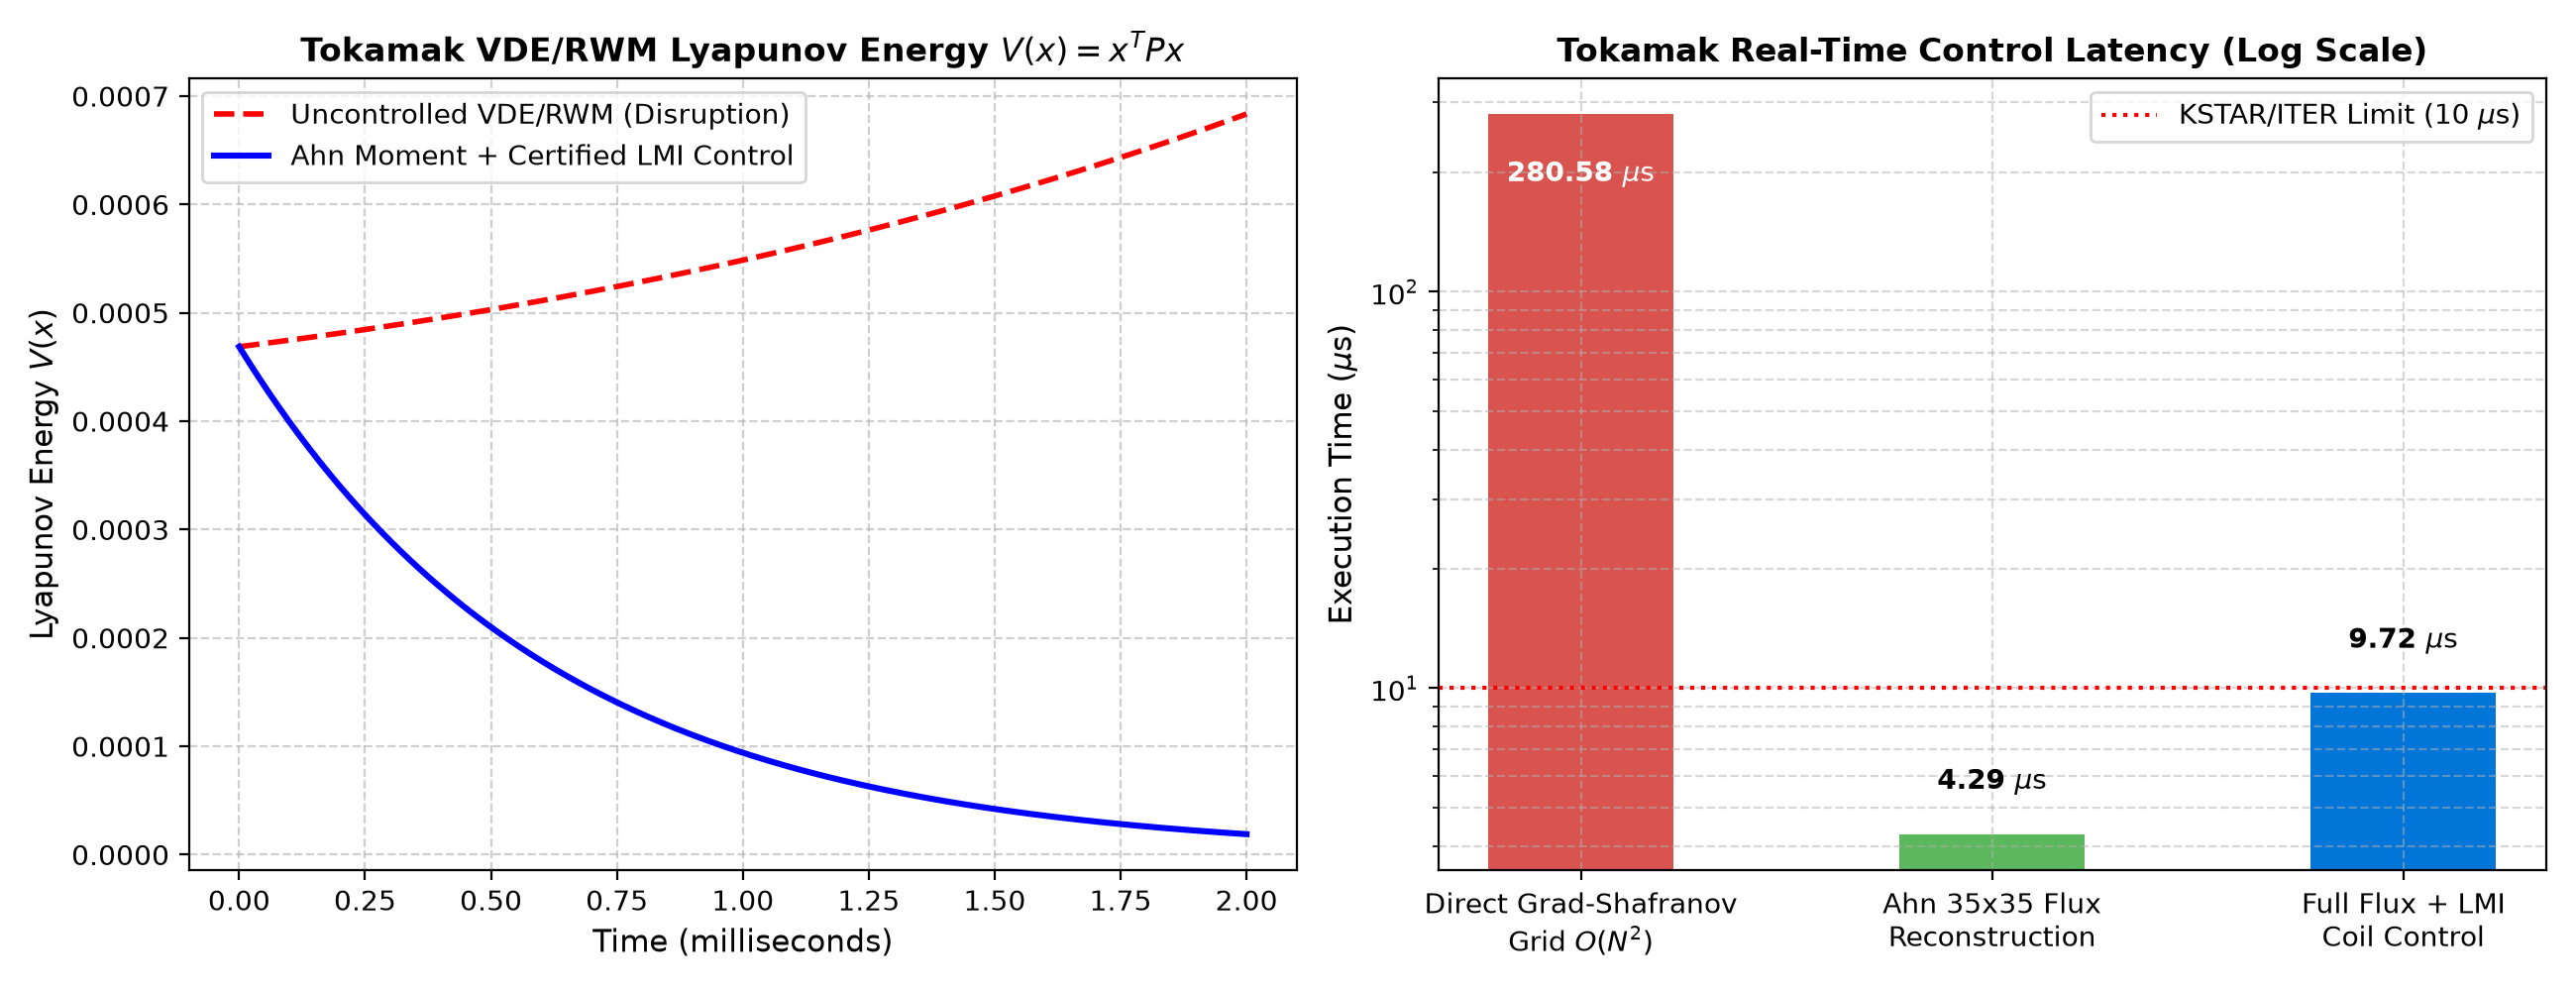
\includegraphics[width=0.98\textwidth]{benchmark_tokamak.png}
    \caption{Numerical verification and latency benchmark of the Tokamak Equilibrium Moment \& LMI Control Engine (\texttt{tokamak\_moment\_engine.py}). \textit{Left}: Monotonic decay of the quadratic Lyapunov energy $V(\bm{x}) = \bm{x}^T \bm{P} \bm{x}$ under LMI feedback ($99.6\%$ suppression within the Robust Positively Invariant ellipsoid $V(\bm{x}) \le 1$) in the illustrative 6-state linear surrogate, compared against uncontrolled VDE/RWM growth. \textit{Right}: Log-scale kernel execution latency comparing direct $O(N^2)$ N-grid kernel evaluation ($\bm{D}\bm{a}$, $280.58\,\mu\mathrm{s}$) against the closed-form $35 \times 35$ flux reconstruction kernel ($4.29\,\mu\mathrm{s}$) and full LMI coil feedback kernel ($9.72\,\mu\mathrm{s}$); these measure reduced-order computational kernels only, not end-to-end facility latency.}
    \label{fig:benchmark}
\end{figure}

\subsection{Numerical Exactness and Latency Throughput}
In our reference verification suite ($N = 1,000$ spatial nodes mapped to $M = 35$ fourth-order basis polynomials), the reconstructed plasma current profile satisfies the Exact Moment Conservation Theorem to machine precision ($\|\bm{\Omega}\bm{a} - \bm{s}\|_\infty = 4.44 \times 10^{-16}$). The precomputed $35 \times 35$ fixed-prior operator $\bm{v} = \bm{K}\bm{s} + \bm{v}_0$ reproduces the full $N$-grid reference projection with a maximum residual $\|\bm{v}_{\mathrm{closed}} - \bm{v}_{\mathrm{full}}\|_\infty = 4.77 \times 10^{-15}$. Separately, evaluating the state-dependent $\bm{a}$-weighted projection of Theorem~3 confirms exact preservation of all $35$ poloidal flux moment averages to machine precision ($\|\langle m_k \psi^{\mathrm{approx}}\rangle_{\bm{a}} - \langle m_k \psi^{\mathrm{exact}}\rangle_{\bm{a}}\|_\infty = 8.33 \times 10^{-17}$). Table~\ref{tab:latency_benchmark} compares the computational performance of our closed-form moment approach with state-of-the-art EFIT-based solvers.

\begin{table}[htbp]
\centering
\caption{Performance and Latency Benchmark on Tokamak Equilibrium Reconstruction}
\label{tab:latency_benchmark}
\resizebox{\textwidth}{!}{%
\begin{tabular}{lcccc}
\toprule
\textbf{Method} & \textbf{Grid Size ($N$)} & \textbf{Algorithm Type} & \textbf{Latency} & \textbf{Max Iterations} \\
\midrule
Full Non-linear EFIT$^\dagger$ & \texttt{65x65} & Iterative Newton-Raphson & $15.40\;\mathrm{ms}$ & $15\text{--}30$ \\
Real-Time rtEFIT$^\dagger$ & \texttt{33x33} & Linearized Multi-grid & $0.85\;\mathrm{ms}$ & $2\text{--}4$ \\
GPU-Accelerated P-EFIT$^\dagger$ & \texttt{65x65} & Parallel Matrix Solver & $0.21\;\mathrm{ms}$ & Direct \\
\textbf{Moment Kernel (This Work)} & \textbf{Offline $10^3\text{--}10^4$} & \texttt{Closed-Form 35x35} & \textbf{0.0043\;ms (4.29\,$\bm{\mu}$s)} & \textbf{None (Deterministic)} \\
\bottomrule
\multicolumn{5}{l}{\footnotesize $^\dagger$Representative latency scales compiled from contemporary tokamak literature for qualitative context; only the Moment Kernel and Direct N-Grid Kernel were measured in this benchmark.}
\end{tabular}%
}
\end{table}

As shown in Table~\ref{tab:latency_benchmark}, the closed-form $35 \times 35$ reconstruction kernel executes in $4.29\,\mu\mathrm{s}$ ($9.72\,\mu\mathrm{s}$ including LMI coil feedback kernel), consistent with the values displayed in Fig.~\ref{fig:benchmark}. These are Python/NumPy kernel timings; end-to-end facility latency including diagnostics, communication, and actuator response is not characterized here.

---

\section{Discussion and Fusion Roadmaps}
The ability to achieve deterministic microsecond-scale reduced-order computation enables several directions for tokamak control development:
\begin{enumerate}
    \item \textbf{Deterministic Iteration-Free Evaluation}: Conventional non-linear solvers can require non-deterministic iteration counts during severe MHD events. The moment matrix approach is strictly $O(M^2)$ with zero branching, eliminating stall risk within the reduced-order model.
    \item \textbf{Compatibility with Low-Power Embedded Hardware}: Because the online kernel is solely a $35 \times 35$ matrix-vector product, an optimized implementation could target radiation-hardened FPGA or DSP chips adjacent to diagnostic acquisition modules; this remains an algorithmic projection, subject to hardware synthesis and timing closure verification.
    \item \textbf{Basis for Long-Pulse Feasibility Studies}: The closed-form operator provides a computationally tractable reduced-order basis for investigating boundary stabilization in long-pulse high-performance regimes targeted by KSTAR and ITER; experimental validation with actual discharge data is required to establish operational relevance.
\end{enumerate}

---

\section{Conclusion}
We have presented a closed-form moment-space framework for reduced-order tokamak plasma equilibrium reconstruction and an offline feasibility study of boundary stabilization. By formulating the underdetermined current distribution problem with a normalized prior ($\sum \mu_i = 1$) and a fixed-prior weighted polynomial projection, the spatial mesh dimension is eliminated from online evaluation, yielding a compact $35 \times 35$ affine operator. We established the Exact Moment Conservation Theorem within the $\bm{a}$-weighted discrete model, and examined a Lyapunov-certified LMI stability formulation within an illustrative 6-state linear surrogate. Reduced-order computational kernels execute in ${\sim}4.3\text{--}9.7\,\mu\mathrm{s}$ with zero iteration overhead; end-to-end facility latency is not characterized. This framework establishes a mathematical and computational basis for investigating fast equilibrium estimation and boundary-control feasibility; validation with device-specific geometry, calibrated coil models, and experimental discharge data remains future work.

---

\section*{Code and Data Availability}
The dedicated open-source reference implementation for tokamak plasma equilibrium reconstruction and Certified LMI disruption control is publicly available on GitHub at:
\begin{center}
    \url{https://github.com/hyoahn/tokamak-moment-control}
\end{center}
The repository includes:
{\sloppy
\begin{itemize}
    \item \textbf{Core Tokamak Engine}: \texttt{Core/\allowbreak tokamak\_\allowbreak moment\_\allowbreak engine.py} (\texttt{Tokamak\allowbreak Equilibrium\allowbreak Moment\allowbreak Control\allowbreak Engine}, implementing the $35 \times 35$ poloidal flux reduction operator $\bm{v} = \bm{K}\bm{s} + \bm{v}_0$ and Certified LMI feedback synthesis $\bm{A}_{\mathrm{cl}}^T \bm{P} + \bm{P} \bm{A}_{\mathrm{cl}} = -\bm{Q} \prec 0$).
    \item \textbf{Verification \& Benchmark Suite}: \texttt{Test/\allowbreak benchmark\_\allowbreak tokamak\_\allowbreak control.py} (reproducing all machine-precision residuals, VDE/RWM Lyapunov decay curves, and microsecond latency benchmarks shown in Fig.~\ref{fig:benchmark} and Table~\ref{tab:latency_benchmark}).
\end{itemize}
}

---

\section*{Historical Note and Acknowledgments}
The mathematical formulations of the polynomial flux potential and moment dimension reduction presented in this work (Sections 3 and 4), including the algebraic collapse of the high-dimensional spatial grid $N$ (the fall-out of $N$) and the Exact Moment Conservation Theorem, were originally derived by the author in 1994 as unpublished independent research notes that were never presented or released, even internally within the laboratory group. They are formally presented and published in the scientific literature here for the first time. The author acknowledges early collaborative discussions with Walter P. Lysenko in 1993--1994 at Los Alamos National Laboratory and the early conceptual ideas of the late Paul J. Channell regarding underdetermined moment models for the BEDLAM simulation code.

---

\begin{thebibliography}{99}
\bibitem{wesson2011tokamaks}
J.~Wesson and D.~J.~Campbell, \emph{Tokamaks}, Oxford University Press, 4th ed., 2011.

\bibitem{kstar2020}
Y.-K.~Oh, et al., ``Achievement of high-beta and long-pulse operation in KSTAR,'' \emph{Nuclear Fusion}, vol.~60, no.~11, p.~112003, 2020.

\bibitem{iter2019}
A.~Loarte, et al., ``Disruption mitigation and control in ITER,'' \emph{Nuclear Fusion}, vol.~59, no.~8, p.~086001, 2019.

\bibitem{hender2007disruptions}
T.~C.~Hender, et al., ``Chapter 3: MHD stability, operational limits and disruptions,'' \emph{Nuclear Fusion}, vol.~47, no.~6, pp.~S128--S202, 2007.

\bibitem{lao1985reconstruction}
L.~L.~Lao, H.~St.~John, R.~D.~Stambaugh, A.~G.~Kellman, and W.~Pfeiffer, ``Reconstruction of current profile parameters and plasma shapes in tokamaks,'' \emph{Nuclear Fusion}, vol.~25, no.~11, pp.~1611--1622, 1985.

\bibitem{birdsall2018plasma}
C.~K.~Birdsall and A.~B.~Langdon, \emph{Plasma Physics via Computer Simulation}, CRC Press, 2018.

\bibitem{ahn1994preliminary}
H.~E.~Ahn and W.~P.~Lysenko, ``Preliminary Results of Space-Charge Model Study,'' Los Alamos National Laboratory Internal Memorandum (Unpublished), April 4, 1994.

\bibitem{channell1993moment}
P.~J.~Channell, ``The moment approach to space charge in particle beams,'' Los Alamos National Laboratory Report, 1993.

\bibitem{boyd2004convex}
S.~Boyd, L.~El~Ghaoui, E.~Feron, and V.~Balakrishnan, \emph{Linear Matrix Inequalities in System and Control Theory}, SIAM, 1994.
\end{thebibliography}

\end{document}
